\documentclass[conference]{IEEEtran}
\usepackage{cite,amsmath,amssymb,graphicx,booktabs,xcolor,tikz,pgfplots}
\usetikzlibrary{arrows.meta,positioning,fit,calc}
\pgfplotsset{compat=1.18}
\newcommand{\tbd}[1]{\textcolor{red}{\textbf{[#1]}}}
\newcommand{\name}{\textsc{PhaSched}}

\begin{document}

\title{Late Breaking Results: Round-Phase-Aware Memory Scheduling for Federated Learning Clients}

\author{\IEEEauthorblockN{Anonymous Author(s)}
\IEEEauthorblockA{Submitted for double-blind review}}

\maketitle

\begin{abstract}
The main-memory traffic of a federated learning (FL) client follows the round structure of the protocol: the network interface writes the global model into DRAM, the cores read and update it during local training, and the network interface reads the update back out. Existing memory schedulers are unaware of these phases and apply a single policy throughout. We propose \name{}, which exposes a 2-bit round-phase register to the memory controller and uses it to select among lightweight presets of an FR-FCFS scheduler. \name{} needs no per-thread state. Evaluated in DAMOV-SIM on four dense-model FL clients, it reduces round time by 0.4\% on average (up to 1.1\%) and average training read latency by 1.2\% (up to 2.8\%) over FR-FCFS, and never lengthens a round.
\end{abstract}

\begin{IEEEkeywords}
federated learning, memory controller, DRAM scheduling, edge computing
\end{IEEEkeywords}

\section{Introduction}
Federated learning (FL) trains a shared model across many clients without moving their data~\cite{fedavg}. In every round a client downloads the global model, trains it on local data and uploads an update. Systems work on FL clients has concentrated on communication cost and on compute heterogeneity~\cite{flscale,flopen}; how a round stresses main memory has received little attention.

We observe that an FL round imposes three distinct and \emph{predictable} traffic patterns on the memory controller (Fig.~\ref{fig:overview}, top). In \textbf{ingress}, the NIC writes the model, tens of megabytes, into DRAM by DMA: a sequential, write-only burst. In \textbf{train}, the cores read weights and activations and write gradients and updated weights; reads dominate and determine progress. In \textbf{egress}, the NIC reads the update out of DRAM: a sequential, read-only stream.

A conventional controller uses FR-FCFS~\cite{frfcfs} with a fixed write-drain policy. Thread-aware schedulers such as PAR-BS~\cite{parbs}, ATLAS~\cite{atlas}, TCM~\cite{tcm} and BLISS~\cite{bliss} improve fairness and throughput across competing threads, and learning-based controllers~\cite{rlsched} adapt reactively. None of them is told what the application already knows exactly: which phase of the round it is in. As a result a single write-drain policy must serve both the bulk NIC transfers and local training, where gradient and weight write-backs interleave with the reads that determine progress: in our measurements training issues one bus turnaround every nine requests and its average read latency is 2.7$\times$ that of a read-only stream.

\textbf{Contribution.} We propose \name{}, a phase-aware extension of FR-FCFS in which the FL runtime announces the current round phase to the memory controller, and the controller switches to a preset tuned for that phase. The mechanism costs a 2-bit register and a four-entry preset table, and requires four register writes per round.

\begin{figure}[t]
\centering
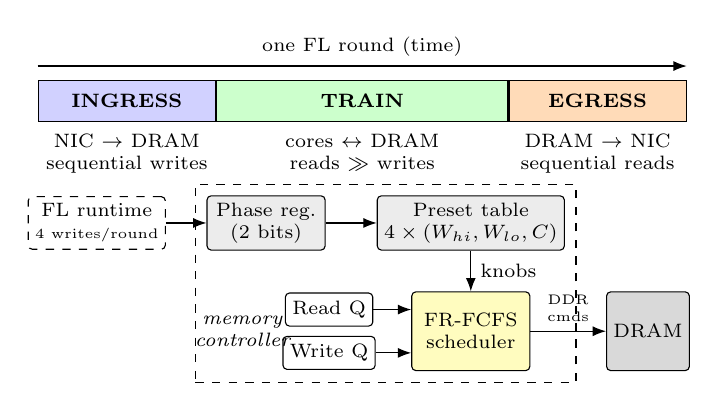
\begin{tikzpicture}[font=\scriptsize,>=Latex,
  ph/.style={draw,minimum height=0.52cm,inner sep=1pt},
  blk/.style={draw,rounded corners=1.5pt,minimum height=0.55cm,align=center,inner sep=2.5pt}]
\node[ph,fill=blue!18,minimum width=2.25cm,anchor=west] (ing) at (-0.75,0) {\textbf{INGRESS}};
\node[ph,fill=green!20,minimum width=3.7cm,right=0pt of ing] (trn) {\textbf{TRAIN}};
\node[ph,fill=orange!28,minimum width=2.25cm,right=0pt of trn] (egr) {\textbf{EGRESS}};
\node[below=1pt of ing,align=center] (ingl) {NIC $\rightarrow$ DRAM\\sequential writes};
\node[below=1pt of trn,align=center] (trnl) {cores $\leftrightarrow$ DRAM\\reads $\gg$ writes};
\node[below=1pt of egr,align=center] (egrl) {DRAM $\rightarrow$ NIC\\sequential reads};
\draw[->] ([yshift=5pt]ing.north west) -- node[above,pos=0.5]{one FL round (time)} ([yshift=5pt]egr.north east);
\node[blk,dashed,minimum width=1.45cm] (rt) at (0,-1.55) {FL runtime\\{\tiny 4 writes/round}};
\node[blk,fill=gray!15,minimum width=1.5cm] (reg) at (2.15,-1.55) {Phase reg.\\(2 bits)};
\node[blk,fill=gray!15,minimum width=2.3cm] (tab) at (4.75,-1.55) {Preset table\\$4\times(W_{hi},W_{lo},C)$};
\node[blk,minimum width=1.05cm,minimum height=0.42cm] (rq) at (2.95,-2.65) {Read Q};
\node[blk,minimum width=1.05cm,minimum height=0.42cm] (wq) at (2.95,-3.2) {Write Q};
\node[blk,fill=yellow!25,minimum width=1.5cm,minimum height=1.0cm] (sch) at (4.75,-2.925) {FR-FCFS\\scheduler};
\node[blk,fill=gray!30,minimum width=0.9cm,minimum height=1.0cm] (dram) at (7.0,-2.925) {DRAM};
\draw[->] (rt) -- (reg);
\draw[->] (reg) -- (tab);
\draw[->] (tab) -- node[right]{knobs} (sch);
\draw[->] (rq.east) -- (rq.east -| sch.west);
\draw[->] (wq.east) -- (wq.east -| sch.west);
\draw[->] (sch) -- node[above,font=\tiny,align=center]{DDR\\cmds} (dram);
\node[draw,dashed,inner sep=4pt,fit=(reg)(tab)(sch)(rq)(wq)] (mc) {};
\node[align=center,font=\scriptsize\itshape] at (1.85,-2.925) {memory\\controller};
\end{tikzpicture}
\caption{Top: memory traffic of one FL round on a client. Bottom: \name{}. The FL runtime writes the current phase; the phase selects the write-drain watermarks $W_{hi}$, $W_{lo}$ and the row-hit streak cap $C$ used by an otherwise unmodified FR-FCFS scheduler.}
\label{fig:overview}
\end{figure}

\section{\name{}}
\subsection{Phase Interface}
The controller holds a register $\textsc{phase}\in\{\textsc{idle},\textsc{ingress},\textsc{train},\textsc{egress}\}$. The FL runtime updates it through a privileged register write at the three points where the round changes character: before it starts receiving the model, before it starts local training, and before it starts sending the update; a fourth write returns it to \textsc{idle} at the end of the round.
These points already exist as distinct calls in FL frameworks, so no application restructuring is needed. When the register holds \textsc{idle}, the controller behaves exactly as the baseline, so non-FL software is unaffected.

\subsection{Phase Presets}
\name{} does not introduce a new scheduling algorithm. It re-tunes three knobs that an FR-FCFS controller already has: the high and low write-queue watermarks $W_{hi}$ and $W_{lo}$, which decide when the controller enters and leaves write-drain mode, and the cap $C$ on consecutive row hits served before an older request to another row is considered. Table~\ref{tab:presets} lists the presets.

\begin{table}[t]
\centering
\caption{Phase presets of \name{}}
\label{tab:presets}
\footnotesize
\begin{tabular}{@{}llll@{}}
\toprule
Phase & Write drain & Cap $C$ & Intent \\
\midrule
\textsc{idle} & baseline & baseline & unchanged \\
\textsc{ingress} & eager (queue non-empty) & unlimited & long write bursts \\
\textsc{train} & baseline $+$ age bound $T_{max}$ & baseline & no write backlog \\
\textsc{egress} & only at $W_{hi}$ & unlimited & long read runs \\
\bottomrule
\end{tabular}
\end{table}

\textbf{Ingress} enters write mode as soon as the write queue is non-empty and stays until it is empty; without a row-hit cap, each row of the sequential DMA stream is activated once and written completely.

\textbf{Train} keeps the baseline watermarks and cap, so writes drain in batches, but bounds their age: a write older than $T_{max}$ triggers a drain, so no backlog later blocks reads in a long burst. Leaving write mode whenever a read arrives performed worse: it splits drains into short bursts that each pay a turnaround.

\textbf{Egress} keeps the controller in read mode without a row-hit cap, serving the NIC stream in long row-hit runs; residual writes drain only at $W_{hi}$.

\textbf{Starvation guard.} In every FL phase, a request older than $T_{max}=2000$ DRAM cycles (1.7\,$\mu$s) is served next, switching queues if needed; this bounds the delay of traffic that does not match the phase, e.g., a co-running application.

\textbf{Cost.} A 2-bit register, a four-entry table of watermark and cap values and multiplexers on three existing comparators: fewer than 100 bits of state. Unlike ATLAS, TCM or BLISS, \name{} keeps no per-thread counters and performs no ranking.
\section{Evaluation Methodology}
We implement \name{} in DAMOV-SIM~\cite{damov}, which couples ZSim~\cite{zsim} with Ramulator~\cite{ramulator}. \emph{Network model:} DAMOV-SIM has no NIC. We add a DMA injector at the ZSim--Ramulator boundary that issues cache-bypassing write (ingress) and read (egress) requests over the model buffer at the configured link rate. \emph{Phase interface:} a ZSim magic instruction forwards the phase to the Ramulator controller.  \emph{Workloads:} four synthetic FedAvg clients (MLP, CNN, LSTM, GRU) in C++/OpenMP with real forward and backward passes on 256\,MB of local data; the model is one buffer that the DMA injector transfers, and each run simulates one round of $K$ minibatches.
\emph{System and workloads:} Table~\ref{tab:config}. \emph{Baselines:} FCFS, FR-FCFS, FR-FCFS with row-hit cap, and BLISS. \emph{Metrics:} round time and its per-phase breakdown, average and tail read latency, number of read/write bus turnarounds, and DRAM energy.

\begin{table}[t]
\centering
\caption{Simulated configuration}
\label{tab:config}
\footnotesize
\begin{tabular}{@{}ll@{}}
\toprule
Cores & 4 $\times$ 4-wide out-of-order x86-64, 2.4\,GHz \\
Caches & 32\,kB L1, 256\,kB L2, 8\,MB shared L3 \\
Memory & DDR4-2400, 1 channel, 1 rank, 32-entry read/write queues \\
Network & 10\,GbE (1.25\,GB/s), modelled by the DMA injector \\
Workloads & FedAvg clients: MLP 1024-2048-2048-10 (24\,MB); \\
 & CNN 2$\times$conv3$\times$3 + 2 FC, 32$\times$32 images (32\,MB); \\
 & 2-layer LSTM / GRU, hidden 512 (14 / 11\,MB) \\
Round & one round; $K$=2/2/1/1 minibatches of \\
 & 32/16/8/8 samples (MLP/CNN/LSTM/GRU) \\
\bottomrule
\end{tabular}
\end{table}

\section{Preliminary Results}
Fig.~\ref{fig:results} shows round time normalised to FR-FCFS. \name{} shortens the round by 0.4\% on average (geometric mean; up to 1.1\%, MLP) and is never slower than FR-FCFS. At 10\,GbE, ingress and egress are link-bound and equal under all schedulers; the gain comes from training, where write-backs compete with reads: average read latency falls by 1.2\% (up to 2.8\%, GRU) and the MLP's median read latency by 20\%. Scheduling matters on these clients: FCFS lengthens the round by 7.6\%, the row-hit cap by 0.9\% and BLISS by 1.1\%, confirming that thread-level fairness does not capture phase behaviour. DRAM energy, estimated from command counts and DDR4 datasheet currents, falls by 0.4\% (up to 1.2\%, MLP), with up to 11\% fewer row activations.

\begin{figure}[t]
\centering
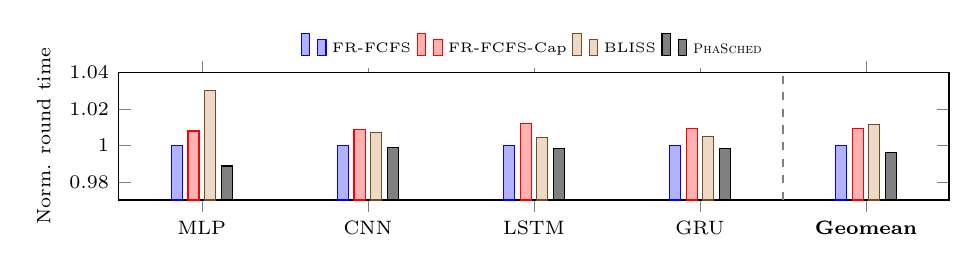
\begin{tikzpicture}
\begin{axis}[ybar,width=\columnwidth,height=3.2cm,ymin=0.97,ymax=1.04,ytick={0.98,1.00,1.02,1.04},yticklabel style={/pgf/number format/fixed,/pgf/number format/precision=2},
  ylabel={Norm. round time},ylabel style={font=\scriptsize},
  xtick={1,2,3,4,5},xticklabels={MLP,CNN,LSTM,GRU,\textbf{Geomean}},xmin=0.5,xmax=5.5,
  tick label style={font=\scriptsize},enlarge x limits=false,bar width=4pt,
  legend style={font=\tiny,at={(0.5,1.03)},anchor=south,legend columns=4,draw=none}]
\addplot coordinates {(1,1) (2,1) (3,1) (4,1) (5,1)};
\addplot coordinates {(1,1.0079) (2,1.0087) (3,1.0120) (4,1.0094) (5,1.0095)};
\addplot coordinates {(1,1.0301) (2,1.0071) (3,1.0042) (4,1.0047) (5,1.0115)};
\addplot coordinates {(1,0.9887) (2,0.9988) (3,0.9984) (4,0.9985) (5,0.9961)};
\draw[gray,dashed,thin] (axis cs:4.5,0.97) -- (axis cs:4.5,1.04);
\legend{FR-FCFS,FR-FCFS-Cap,BLISS,\name{}}
\end{axis}
\end{tikzpicture}
\caption{Round time normalised to FR-FCFS (lower is better; y-axis from 0.97). Geomean (right of the dashed line): geometric mean.}
\label{fig:results}
\end{figure}

\section{Conclusion and Ongoing Work}
An FL round tells the system in advance what its memory traffic will look like; \name{} passes this to the memory controller with a 2-bit hint and re-tunes existing FR-FCFS knobs per phase. Ongoing work covers asynchronous FL, where phases overlap, and predicting the phase inside the controller so that no software hint is needed.

\input{refs_short.bbl}
\end{document}
